        \clearpage
        \begin{figure*}[ht]
            \pdfbookmark[2]{ID 06}{figure_id_06}
        	\centering
            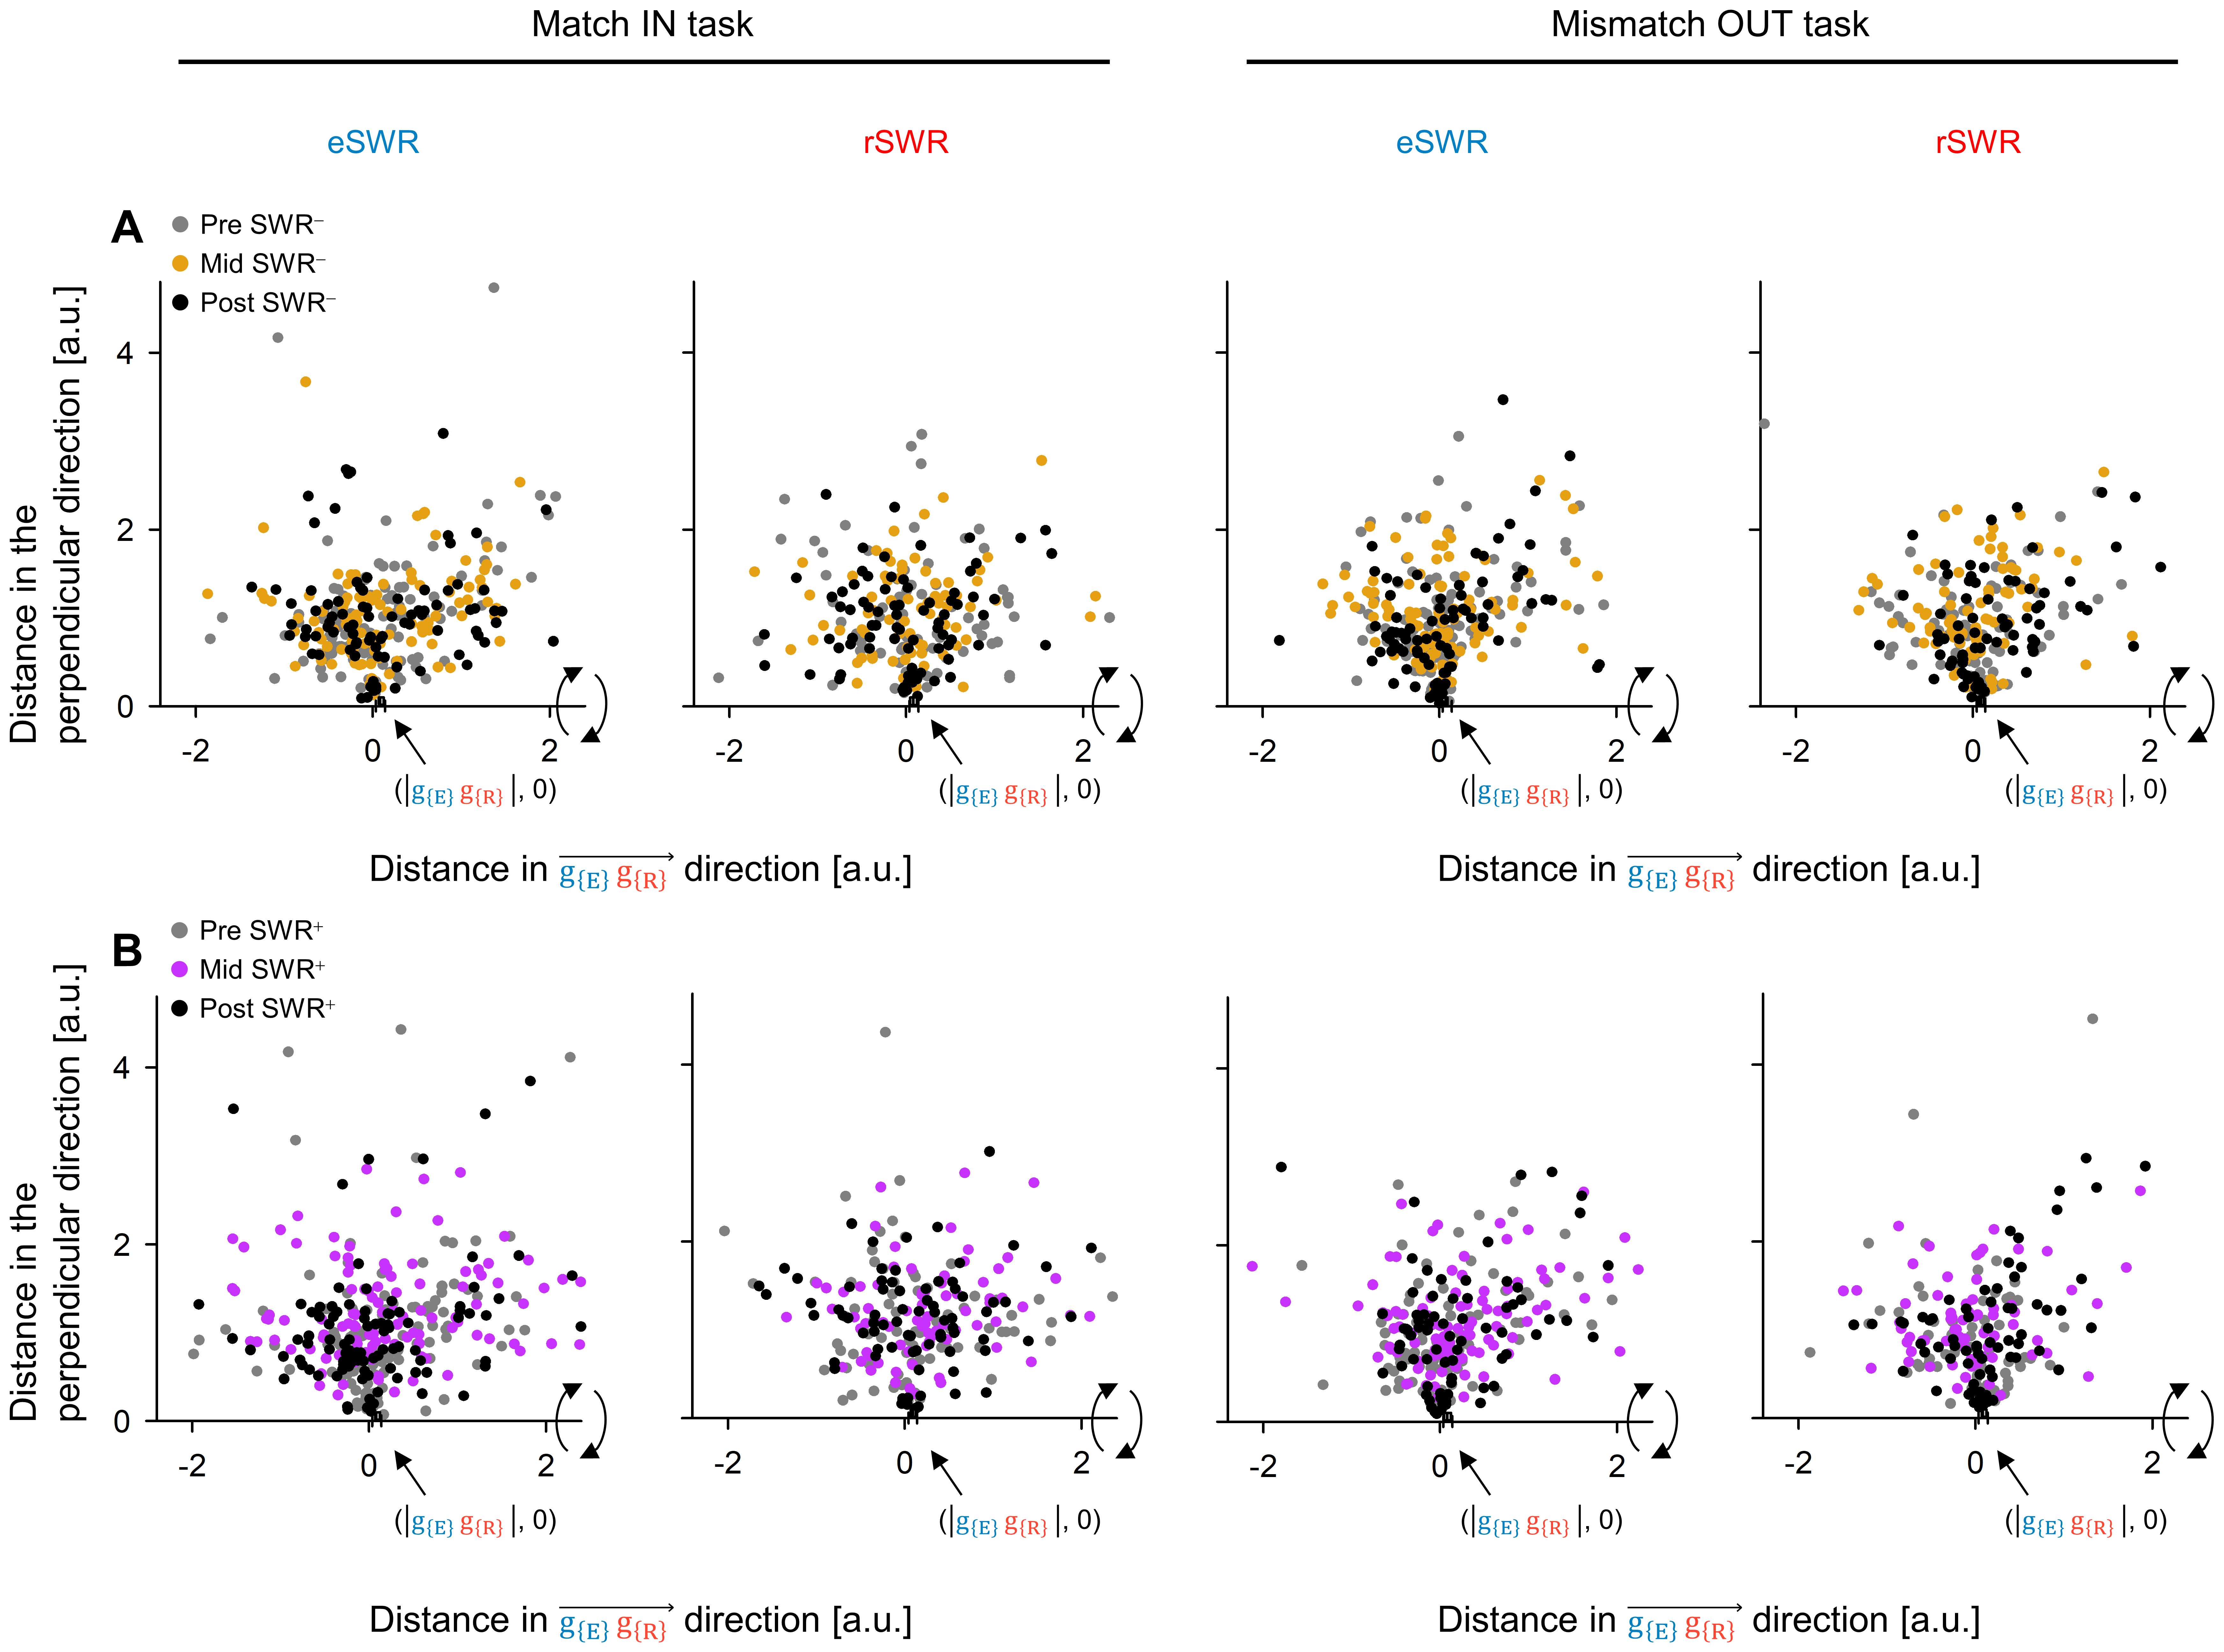
\includegraphics[width=1\textwidth]{./src/figures/.png/Figure_ID_06.png}
        	\caption{\textbf{
Visualizing Neural Trajectory During SWR in Two-Dimensional Space
}
\smallskip
\\
The presented neural trajectories pertain to hippocampal activity during Sharp-Wave Ripple (SWR) events, shown in two-dimensional space. \textbf{\textit{A.}} Trajectories representative of pre- (\textit{gray}), mid- (\textit{yellow}), and post-SWR$^-$ (\textit{black}) phases of an SWR event~\cite{buzsaki_hippocampal_2015}. \textbf{\textit{B.}} Trajectories corresponding to SWR$^+$ scenarios in contrast to SWR$^-$~\cite{fernandez-ruiz_long-duration_2019}. The magnitude of $\lVert \mathrm{g_{E}g_{R}} \rVert$ exhibits fluctuations within sessions~\cite{liu_consensus_2022}. The projecting protocol is as follows: initially, $\mathrm{g_{E}}$ was situated at the origin $O$ (0,0), and $\mathrm{g_{R}}$ at ($\lVert \mathrm{g_{E}g_{R}} \rVert$, 0) via linear transformation~\cite{kim_corticalhippocampal_2022}. Subsequently, the point cloud was rotated around the $\mathrm{g_{E}g_{R}}$ axis (the x-axis) to be compatible with a two-dimensional environment~\cite{yu_gaussian-process_2009}. Thus, both the distances from $O$ and the angles with the $\mathrm{g_{E}g_{R}}$ axis remained unaltered from their three-dimensional configuration~\cite{mcinnes_umap_2018}. Abbreviations: SWR represents Sharp-Wave Ripple events; eSWR denotes SWR during the encoding phase; rSWR signifies SWR during the retrieval phase; SWR$^+$ typifies an SWR event; SWR$^-$ signals the control events for SWR$^+$; pre-SWR, mid-SWR, or post-SWR refer to the time interval from $-800$ to $-250$ ms, from $-250$ to $+250$ ms, or from $+250$ to $+800$ ms from the center of the SWR, respectively~\cite{zhang_hippocampal_2022}.
}
% width=1\textwidth
        	\label{fig:06}
        \end{figure*}
